%%%%%%%%%%%%%%%%%%%%%%%%%%%%%%%%%%%%
%% Template file SP 2024
%% Include in directory homework.sty and headerfooter.tex
%%%%%%%%%%%%%%%%%%%%%%%%%%%%%%%%%%%%

\documentclass[12pt]{article}
% \setlength {\marginparwidth }{2cm}
% \setlength{\headheight}{33.40004pt}
\usepackage{homework}

\graphicspath{{images/}}
\geometry{letterpaper, portrait, includeheadfoot=true, hmargin=1in, vmargin=1in}

\setcounter{section}{-1}
%% Solution hiding %%
\usepackage[utf8]{inputenc}
\usepackage{lipsum}


\begin{document}
\singlespacing

\renewcommand{\familydefault}{\rmdefault}
\pagestyle{fancy}
\fancyhf{}
\setlength{\headheight}{30pt}
\renewcommand{\headrulewidth}{0.4pt}
\renewcommand{\footrulewidth}{0.4pt}
\lhead{\large Homework 2 \\ Due Feb. 20, 2024 }
\rhead{\large CS 446 \\ Spring 2024}
\rfoot{\textbf{Page \thepage}}
\lfoot{}

\section{Instructions}

Homework is due Thursday, February 6, 2024 at 23:59pm Central Time.
Please refer to \url{https://courses.grainger.illinois.edu/cs446/sp2024/homework/hw/index.html} for course policy on homeworks and submission instructions.

\section{Short answer: 10pts}
\begin{enumerate}
\item $O(MN)$. Each $N$ test image has to be compared to all $M$ training images to get the top $l$ nearest neighbors.
\item 10. Since if the number is too small, the predicted label will be too easily to change.
\item $\omega = (1, 1)^{T}$, $b = 0$. 
\item The largest eigenvalue of $A^{T}A$ is the square of the largest singular value of $A$.
\item Text data. Since real world text data often involves sequential relationships between words and paragraphs, which violates the iid assumption.
\end{enumerate}

\section{Linear Regression: 10pts}
\begin{enumerate}
\item Since $\omega \in \mathbb{R} ^{d}$, thus the number of unkown parameters is $d$. While the rank of the matrix $X$ is $n$, thus the number of valid equations is $n$. Since $n < d$, there are infinite solutions.
\item From the definition of SVD, we know the rank of $\sum $ is the same as $rank(X)=n$. 
\item From the SVD result, we have $XX^{T} = U\Sigma V^{T}V \Sigma U^{T}$, since $V$ is an orthogonal matrix, thus $V^{T}V = I$. Then we have $XX^{T} = U\Sigma\Sigma^{T} U^{T}$. We can view this as an SVD result of $XX^{T}$, thus the rank of $XX^{T}$ is $n$, which means $XX^{T}$ is full rank.
\end{enumerate}

\section{SVM: 10 pts}
\begin{enumerate}
\item 2. Since the dataset is linearly separable, there must be at least two support vectors that each of them is on the margin.
\item The smallest possible number would be 3 and the largest is $n$. Since all positive $\alpha$s must be on the margin, so the smallest number is 3.
      If all data points are on the margin, but their contributions to this solution is 0, then the largest number is $n$.
\item \begin{enumerate}
    \item \begin{eqnarray}
        (x^{T}z+1)^{T}(x^{T}z+1) &=& (z^{T}x+1)(x^{T}z+1) \nonumber
        \\ &=& z^{T}xx^{T}z + z^{T}x + x^{T}z + 1 \nonumber
        \\ &=& (x^{T}z)^{T}x^{T}z + (\sqrt{2} x)^{T}(\sqrt{2} z) + 1 \nonumber
        \\ &=& (x_{1}^{2}, x_{2}^{2}, \sqrt{2}x_{1}, \sqrt{2}x_{2}, 1)^{T} (z_{1}^{2}, z_{2}^{2}, \sqrt{2}z_{1}, \sqrt{2}z_{2}, 1) \nonumber
    \end{eqnarray}
    Thus, the feature map is $\phi(x) = (x_{1}^{2}, x_{2}^{2}, \sqrt{2}x_{1}x_{2}, \sqrt{2}x_{1}, \sqrt{2}x_{2}, 1)$
    \item One solution is $\omega = (0, 0, 1, 0, 0, 0)$
\end{enumerate}

\end{enumerate}

\section{Gaussian Naive Bayes: 15pts}
\begin{enumerate}
    \item From naive bayes equation, we have:
    \begin{eqnarray}
    P(y=1|x) &=& \frac{P(x|y=1)P(y=1)}{P(x)} \nonumber
        \\    &=& \frac{P(x|y=1)p}{P(x|y=1)p + P(x|y=-1)(1-p)} \nonumber
        \\    &=& \frac{1}{1 + \frac{P(x|y=-1)(1-p)}{P(x|y=1)p}} \nonumber
    \end{eqnarray}
    Thus, $A = P(x|y=-1)(1-p)$, $B = P(x|y=1)p$.
    \item From the results of the previous question, we have: \begin{eqnarray}
        \log \frac{A}{B} &=& \log \frac{(1-p)\prod_{j} e^{-\frac{1}{2}(x_{j}-\mu _{-,j})^{2}}}{p\prod_{j} e^{-\frac{1}{2}(x_{j}-\mu _{+,j})^{2}}} \nonumber
        \\ &=& \log \frac{1-p}{p} + \sum_{j} \left( -\frac{1}{2}(x_{j}-\mu _{-,j})^{2} + \frac{1}{2}(x_{j}-\mu _{+,j})^{2} \right) \nonumber
        \\ &=& \log \frac{1-p}{p} + \sum_{j} \frac{1}{2} \left(x_{j}^{2} - 2 x_{j}\mu _{+,j} + \mu _{+,j}^{2} - x_{j}^{2} +2 x_{j}\mu _{-,j} -\mu _{-,j}^{2} \right) \nonumber
        \\ &=& \log \frac{1-p}{p} + \frac{1}{2} (\mathbf{\mu_{-}} - \mathbf{\mu_{+}})^{T}x + \frac{1}{2}(\mathbf{\mu_{+}}^{T}\mathbf{\mu_{+}} - \mathbf{\mu_{-}}^{T}\mathbf{\mu _{-}}) \nonumber
    \end{eqnarray}
    \item From the previous results, we can easily know a similar result for $P(y=-1|x)$:
    \begin{eqnarray}
        P(y=-1|x) &=& \frac{1}{1 + e^{\log\frac{B}{A}}} \nonumber
        \\ &=& \frac{1}{1 + e^{-\log\frac{A}{B}}} \nonumber
        \\ &=& \frac{1}{1 + e^{-(\omega^{T}x+b)}} \nonumber
    \end{eqnarray}
    Combined with $P(y=1|x) = \frac{1}{1+e^{\omega^{T}x+b}}$, we get the single expression: \begin{equation}
        P(y|x) = \frac{1}{1+e^{-y(\omega^{T}x+b)}}
    \end{equation} where $\omega$ and $b$ are as same as the previous question.
\end{enumerate}

\section{Linear regression: 14pts + 1pt}
    \begin{figure}[h]
    \centering
    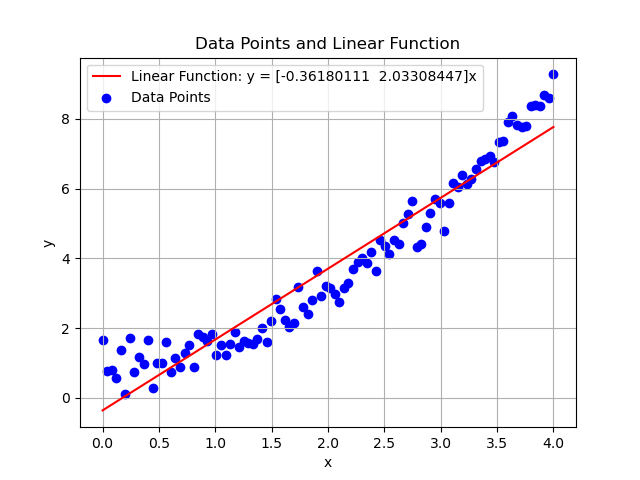
\includegraphics[width=0.5\textwidth]{imgs/Figure_grad.png}
    \caption{Results of the gradient descent method}
    % \label{fig:hw1_6}
    \end{figure}

    \begin{figure}[h]
        \centering
        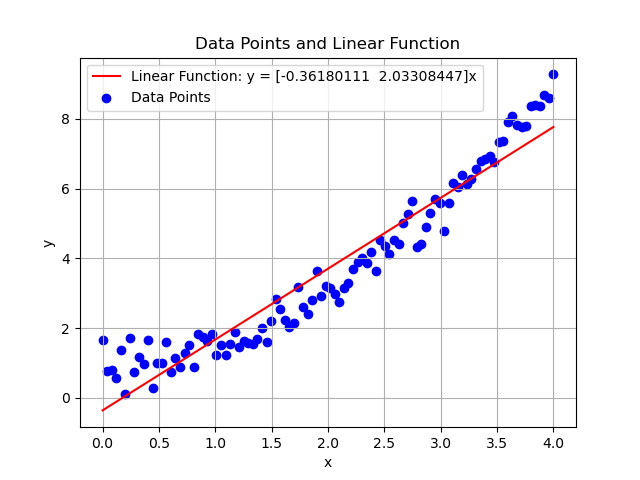
\includegraphics[width=0.5\textwidth]{imgs/Figure_normal.png}
        \caption{Results of the gradient descent method}
        % \label{fig:hw1_6}
        \end{figure}

\end{document}